\documentclass[11pt,a4paper]{article}

\usepackage{amsmath} %for mathemathic formulas
\usepackage{amssymb}
\usepackage[ngerman]{babel} %for the german language by the spellling reform (without the package the date would look like April 20, 2020)
\usepackage{enumitem} %for enumeration surrounding 
\usepackage{graphicx} %for pictures

\title{Blatt 1}
\date{\today}
\author{Hannah Rotgeri \and Feline Heinzelmann}

\begin{document}
    \maketitle

    \section*{Aufgabe 1}
    \begin{itemize}
        \item Beschleunigertypen: \
            \begin{enumerate}[label=(\roman*)]
                \item Elektrostatische Beschleuniger (Cockroft-Walton-Generator über Kondensatoren, Van-de-Graaf-Generator über Ladungstrennung), 
                \item Beschleuniger abhängig von einem zeitlich veränderlichen B-Feld,
                \item HF-Beschleuniger (Linearbeschleuniger und Kreisbeschleuniger z.B. Zyklotron für Protonen und Ionen, Mikrotron für 
                Elektronen, Speicherringe) 
                \item Beschleuniger mit neuen Beschleunigerkonzepten (E-Felder in ultrakurzen Laserpulsen, Plasmawellen, wake-Feldern 
                z.B. Laser-Plasma-Beschleuniger)
            \end{enumerate}
        \item Bewegung im longitudinalen Phasenraum, Phasenfokussierung, momentum compadtion factor (hier: Bewegung im Speicherring)
            \begin{itemize}
                \item Teilchen im Beschleuniger bewegen sich longitudinal um Sollteilchen (hypothetisches Teilchen) in einer 
                Synchrotron-Oszillation
                \item Phasenraum = 2D Raum mit ortsartiger und mit einer impulsartiger Koordinate
                \item Longitudinaler Phasenraum = Bewegung entlang der Strahlrichtung mit 2 Ortskoordinaten (Koordinate s entlang 
                der Bahn im Laborsystem, Koordinate zeitlich relativ zum Sollteilchen im Laborsystem)
                \item Longitudinale Phasenfokussierung = Beeinflussung der Teilchenbahn durch Energieverlust durch Synchrotronstrahlung 
                (Energieabweichung von der Sollbahn um \( \Delta E/E \)) und durch die Teilchenenergie (Änderung der Umlaufzeit durch 
                veränderten Phasenwinkel \(\Phi\): 1. kürzer, wenn Teilchenenergie zunimmt und 2. länger, weil mit der Energie die 
                Bahnlänge zunimmt) \\
                \Rightarrow Folgerung: Auf abfallender Flanke der HF-Spannung \rightarrow kleinerer Energiegewinn \rightarrow Fokussierung 
                des Teilchenstrahls; \\
                Auf ansteigender Flanke der HF-Spannung \rightarrow größerer Energiegewinn \rightarrow Defokussierung 
                \item Mit welcher Flanke würde man Elektronen beschleunigen? Mit der abfallenden Flanke (Bild Phasenwinkel gegen Spannung!!!)
                \item langsame Protonen haben keinen Energieverlust für Protonen aufgrund der hohen Masse 
                \item momentum compaction factor (\( \alpha = \frac{\Delta L /L}{\Delta p /p} \)) = Ableitung der normierten 
                Weglängendifferenz zum normierten Impuls (siehe \ref{fig:phasenfokussierung} und \ref{fig:separatrix})
            \end{itemize}

            \begin{figure}[h]
                \begin{minipage}[t]{0.45\linewidth}
                \centering
                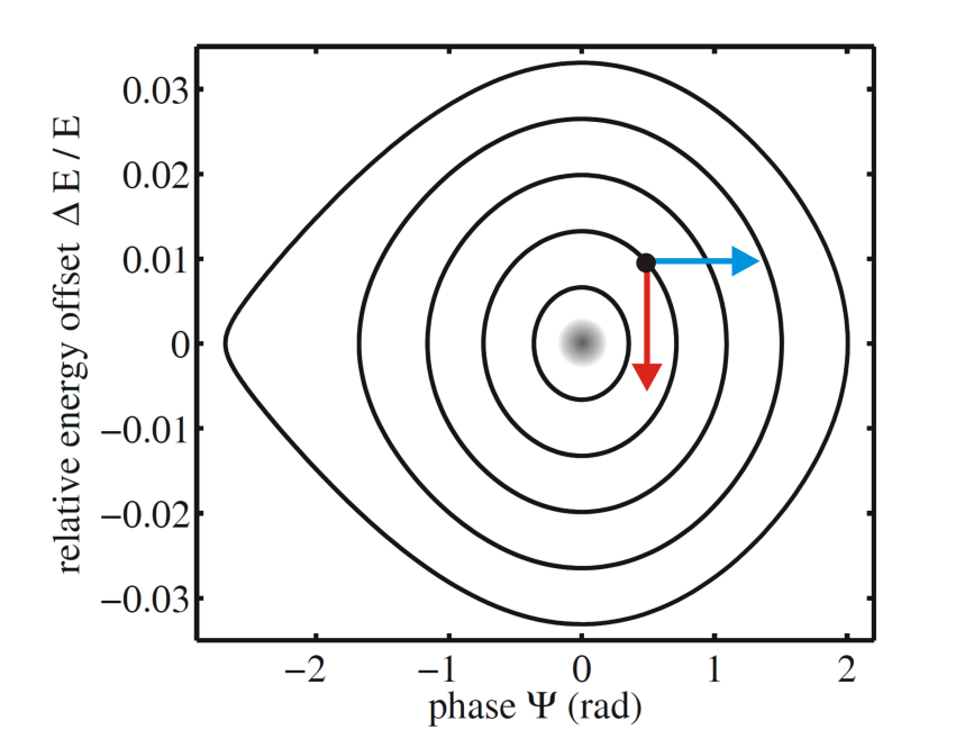
\includegraphics[width=\textwidth]{Longitudinale_Phasenfokussierung_Energie_Phase.PNG} %30% der Textbreite
                \caption{Energie-Phasen-Bild nach einem Umlauf für Elektronen}
                \label{fig:phasenfokussierung}
                \end{minipage}
                \hfill
                \begin{minipage}[t]{0.45\linewidth}
                \centering
                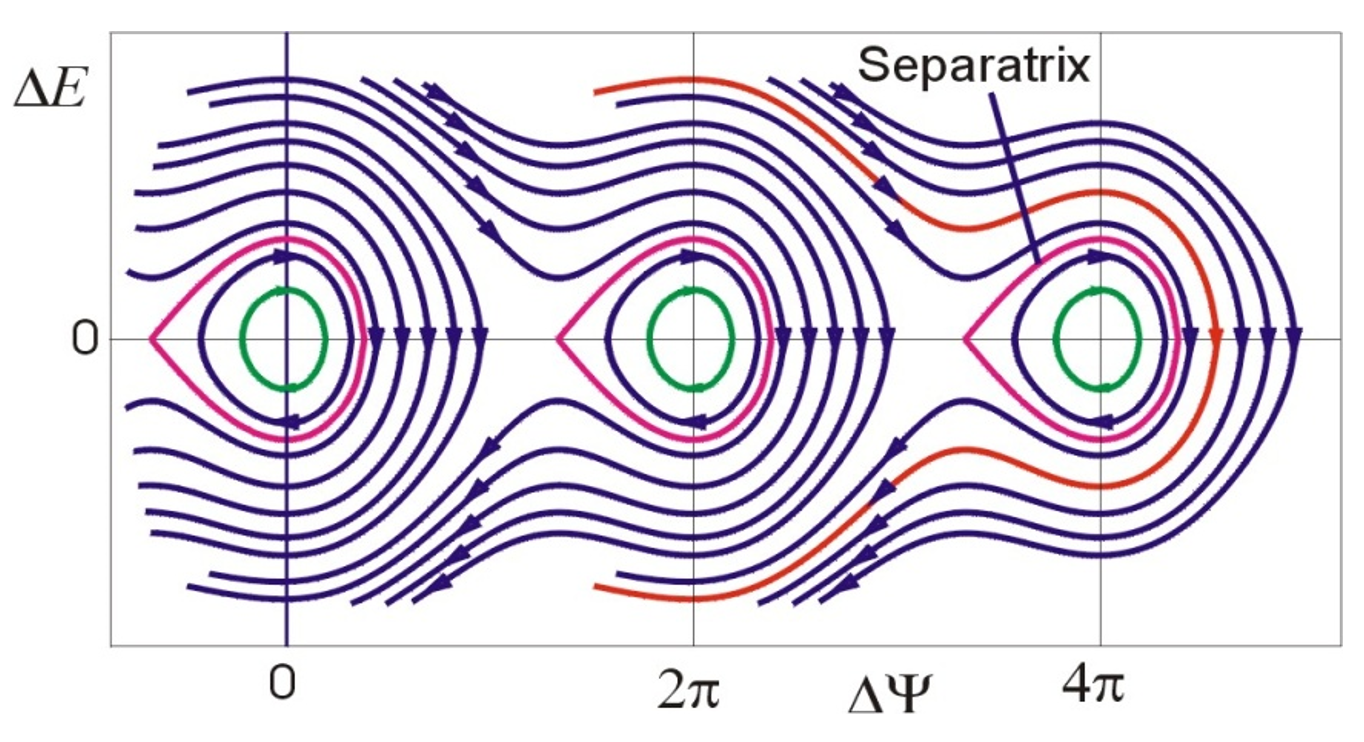
\includegraphics[width=\textwidth]{Longitudinale_Phasenfokussierung_Separatrix.PNG}
                \caption{Energie-Phasen-Bild nach mehreren Speicherringumläufen für Elektronen mit stabilen Bahnen bis zur Grenze, der Separatrix}
                \label{fig:separatrix}
                \end{minipage}
            \end{figure}
            
        \item Bewegungsgleichung im transversalen Phasenraum
            \begin{itemize}
                \item Teilchen im Beschleuniger bewegen sich transversal um Sollteilchen mit einer horizontalen und vertikalen 
                Betatron-Oszillation
                \item Bewegungsgleichungen für bewegte Teilchen im Beschleuniger ähneln denen eines harmonischen Oszillators mit 
                ständig ändernder Frequenz und Amplitude
                \item Transversaler Phasenraum = Bewegung senkrecht zur Strahlrichtung im mitbewegten Koordinatensystem (Koordinate x für horizontale 
                drehende Teilchenbewegung durch horizontale ablenkende Dipolmagnete (sonst konstant horizontale Teilchenbewgungskomponente), 
                Koordinate y für vertikale Teilchenbewegung (hier mit konstanter vertikaler Teilchenbewegungskomponente, da keine vertikal ablenkenden Dipole)
                \item Koordinate \(x \prime \) steht für die örtliche Ableitung nach s (s = Ort des Sollteilchens im Laborsystem)
            \end{itemize}

            \begin{figure}[h]
                \centering
                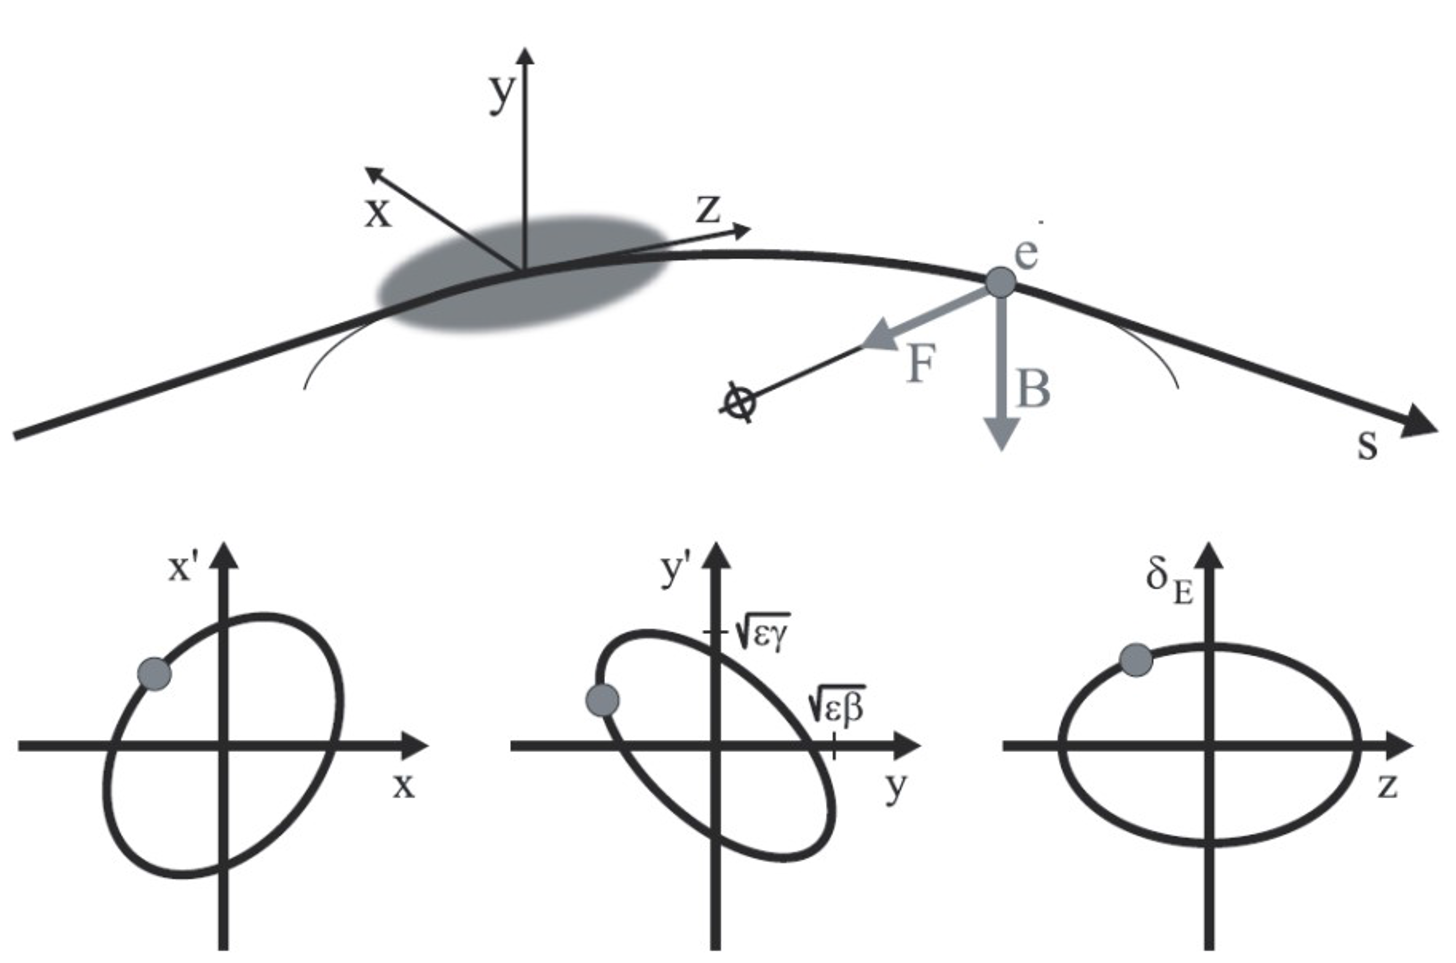
\includegraphics[width=0.7\textwidth]{Phasenraumbewegung.PNG}
                \caption{Phasenraum. Longitudinal: Ort z (und s), Impuls \(\Delta p / \Delta E / \Delta \gamma\); \\ Transversal: Ort x und y, 
                Impuls \( x \prime = \mathrm{d}x/\mathrm{d}s \), \( y \prime = \mathrm{d}y/\mathrm{d}s \) }
            \end{figure}

        \item Transfermatrizen für Driftstrecken, (de)fokussierende Quadrupole, Dipolmagnete
            \begin{itemize}
                \item spezielle Lösungen der Bewegungsgleichungen für Driftstrecken, Quadrupole, Dipole, Sextupole
                \item ähnlich den sog. ABCD-Matrizen in der Optik
                \item sie werden auf Vektoren mit Phasenraumkoordinaten an einer Position, z.B. s = 0, angewandt und ergeben die 
                Phasenraumkoordinaten an einem anderen Ort
            \end{itemize}
        \item Optische Funktionen \( \alpha(s), \beta(s), \gamma(s), D(s),  D(s) \prime \) und ihre Transformation von einem Ort zum anderen
            \begin{itemize}
                \item dazu zählen die Twiss-Paramter und die Dispersionfunktion mit ihrer Ableitung 
            \end{itemize}
        \item Ellipsen im transversalen Phasenraum
            \begin{itemize}
                \item Form durch Twiss-Parameter gegeben, mit konstanter Fläche \( \pi*\epsilon \)
                \item Beschelunigte Teilchen bewegen sich auf der Kante der Ellipse, bei Anwendung der Transfermatrizen 
                ändert sich die Form der Ellipse, Elektron bleibt aber auf Ellipsenkontur
            \end{itemize}
            
            \begin{figure}[h]
                \centering
                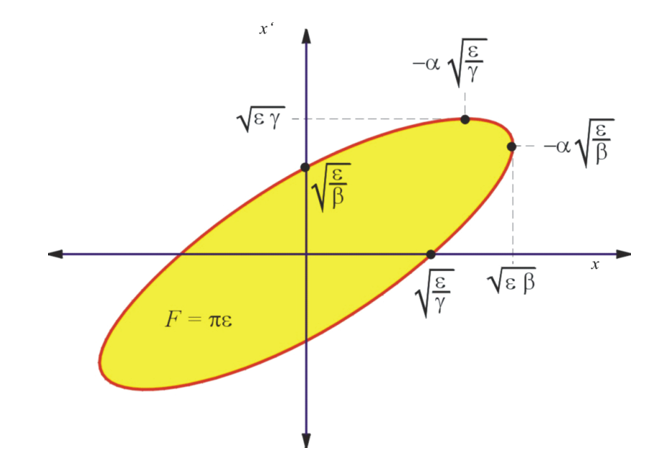
\includegraphics[width=0.7\textwidth]{Ellipse_transversaler_Phasenraum.PNG}
                \caption{Ellipse im transversalen Phasenraum}
            \end{figure}
        \item Ein-Teilchen-Emittanz \( \epsilon \)
            \begin{itemize}
                \item auch sogenannte Courant-Snyder-Invariante
                \item ist für jedes Teilchen verschieden, aber ortsinvariant
                \item eingeschlossene Fläche der Ellipse im transversalen Phasenraum
            \end{itemize}
        \item Emittanz eines Teilchenstrahls
            \begin{itemize}
                \item Maß für Querschnitt und Bündelung eines Teilchenstrahls in einem Beschleuniger \rightarrow wichtiges Maß
                für die Qualität eine Teilchenstrahls 
                \item abhängig von Größe und Öffnungswinkel des Strahls 
                \item ergibt sich durch Parametrisierung der Einhüllenden eines Ionen- oder Elektronenstrahls im transversalen Phasenraum als 
                zeitlich konstante Ellipse mit \( \epsilon = \gamma*x^2 + 2\alpha*x (x \prime)^2 + \beta*(x \prime)^2 \) und \( \alpha, \beta, \gamma \)
                als optische Funktionen (sog. Twiss-Parameter)
                \rightarrow \( \epsilon \) als Volumen, das ein Teilchenstrahl/Lichtstrahl im Phasenraum einnimmt 
            \end{itemize}
        \item Dispersion
            \begin{itemize}
                \item horizontale Ablage aufgrund des abweichenden Bahnradius normiert auf die relative Impulsabweichung \( \Delta p/p \) \( x(s) / \Delta p /p \)
                \item Folge der Impulsabweichung bzw. der Dispersion ist die Änderung des Umfangs der Bahn, gegeben durch den momentum compaction factor
            \end{itemize}
        \item Chromazität und Sextupole
            \begin{itemize}
                \item Chromazität = Änderung des Arbeitspunkts \( \Delta Q\) normiert auf die relative Impulsabweichung 
                (Arbeitspunkt Q = Anzahl der Betatronschwingungen pro Umlauf)
                \item große Chromatizität = großer Fleck im Arbeitspunktdiagramm
                \item negative Chromatizität begünstigt die sog. head-tail-Instabilität
                \item natürliche Chromatizität ist negativ, Korrektur durch (chromatische) Sextupole (\(D \neq 0\)) möglich, die wie ortsabhängige 
                Quadrupole wirken
                \item Sextupole müssen im Beschleuniger an Punkten mit (\(D \neq 0\)) angeordnet section
            \end{itemize}
        \item Fodostruktur und Achromat
            \begin{itemize}
                \item abwechselnd fokussierende und defokussierende Magnetstrukturen, kurz AG-Fokussierung (horizontal fokussierender Quadrupol, Driftstrecke, 
                horizontal defokussierender Quadrupol, Driftstrecke)
                \item ohne Fodostruktur gäbe es im Betatron nur eine schwache Fokussierung durch das B-Feld 
                \rightarrow große Betratron-Oszillationsamplitude \rightarrow große Apertur
                \item Analogon zur Optik mit abwechselnder Folge von Sammel- und Zerstreuungslinsen
                \item Achromat = in der Optik Linsensystem bestehend aus mindestens zwei Linsen, die unterschiedliche Brechkraft und entgegengesetzte 
                Dispersion besitzen und durch die für zwei Farben die chromatische Aberration (= Abbildungsfehler, weil Licht mit seinen 
                verschiedenen Wellenlängen unterschiedlich stark gebrochen werden) minimiert wird; in der Beschleunigerphysik wechseln sich Achromate
                mit dispersionslosen geraden Strecken ab
                \item Was heißt Dispersion gleich 0 im Zusammenhang von Beschleuniger-Achromaten?
            \end{itemize}
    \end{itemize}
\end{document}